\documentclass{article}

\usepackage{fancyhdr}
\usepackage{extramarks}
\usepackage{amsmath}
\usepackage{amsthm}
\usepackage{amsfonts}
\usepackage[plain]{algorithm}
\usepackage{algpseudocode}
\usepackage{matlab-prettifier}
\usepackage{graphicx}
\usepackage[export]{adjustbox}
%
% Basic Document Settings
%
\lstMakeShortInline[style=Matlab-editor]"

\topmargin=-1in
\evensidemargin=0in
\oddsidemargin=0in
\textwidth=6.5in
\textheight=9.0in
\headsep=0.25in

\linespread{1.1}


\rhead{\firstxmark}
\lfoot{\lastxmark}
\cfoot{\thepage}

\renewcommand\headrulewidth{0.4pt}
\renewcommand\footrulewidth{0.4pt}

%
% Homework Details
%   - Title
%   - Due date
%   - Class
%   - Section/Time
%   - Instructor
%   - Author
%

\newcommand{\hmwkTitle}{AMATH 482 Homework 2: G\'abor transforms}
\newcommand{\hmwkDueDate}{January 25, 2019}
\newcommand{\hmwkClassInstructor}{Professor Nathan Kutz}
\newcommand{\hmwkAuthorName}{\textbf{Skyler Hallinan}}

%
% Title Page
%

\title{
    \textmd{\textbf{\text{ } \hmwkTitle}}\\
}

\author{\hmwkAuthorName}
\date{}

\begin{document}
\maketitle

\section*{\fontsize{19}{15}\selectfont Abstract}
	We started with data (music) in the time domain. Using the Gabor transform, we were able to translate this data into the time and frequency domain, creating a spectogram that allows us to visualize frequencies at specific points in time. We experimented with the different parameters used in the transform, and used it to transform to differentiate between the music of a piano and a recorder.
\section*{\fontsize{19}{15}\selectfont Introduction and Overview}
	In data such as music, we often collect it in in the time domain - Although we can tell when things happen, it is hard to tell what is going on in terms of frequencies. The Fourier Transform is a solution lets us transport this data into the frequency domain. However, with this transformed data, we now know what frequencies occur, but we have do not now when they occur in time. The Gabor transform allows us to take small chunks of data across our time domain, which are isolated by multiplying a filter around, then taking the Fourier transform of this data. Combining this frequency data across the small chunks of time allows us to have both a time and frequency visualization of data: We are now able to see what frequencies dominate at each small time interval. \\ \\
	In this project, we will first look at the effects of changing specific paramaters of the Gabor transform, like sampling rate, as well as window size (how much of the entire domain it captures at each timepoint). In addition, we will experiment with other filters other than the standardly used Gaussian one. Finally, we will look at data taken from a recorder and piano, remove the overtones, and then reproduce the music score, and note the differences between the two instruments.
\section*{\fontsize{19}{15}\selectfont Theoretical Background}
	We have seen that the fourier transform is an integral transform that decomposes a time defined function into its frequency components, and is defined by
	\begin{equation} \label{eq:2a}
		F(k) = \frac{1}{\sqrt2\pi} \int_{-\infty}^{\infty} e^{-ikx} f(x) dx
	\end{equation}
		\begin{equation} \label{eq:2b}
		f(x) = \frac{1}{\sqrt2\pi} \int_{-\infty}^{\infty} e^{ikx} F(k) dk
	\end{equation}
	The fast fourier transform, which is accessible in things like MATLAB, assumes that the user is working on a $2\pi$ periodic domain. "fftshift" must be used on the transformed data to undo the shifts naturally incurred by the fast fourier transform algorithm. \\ \\
A downside to the fourier transform is that in changing the domain to the frequency domain, it completely removes all time data from the equation. There is no way to visualize what is going on in terms of a time scale. G\'abor resolved this issue. \\
The Gabor transform is defined by $\mathcal { G } [ f ] ( t , \omega ) = \tilde { f } _ { g } ( t , \omega ) = \int _ { - \infty } ^ { \infty } f ( \tau ) \overline { g } ( \tau - t ) e ^ { - i \omega \tau } d \tau = \left( f , \overline { g } _ { t , \omega } \right)$. We see that this GAabor function localizes signal with the fourier transform over specific small windows of time. The $\tau$ paramater is able to slide the window across the entire domain, resulting in a capturing of both time and frequency domain. Because of the nature of this transform, it is also called the short time fourier transform. \\ \\
There are limitations to this method: It is not possible to have perfect resolution in both the frequency and the time domain; increasing time resolution decreases frequency resolution and vice versa. Just like the Heisenberg Uncertainty Principle, it is impossible to know both of these things at the same time. However, one can adjust the parameters of the transform in order to get more data towards one direction or the other. \\ \\
Wavelets are used in these transforms to highlight specific parts of the signal. Wavelets like the Gaussian and the Mexican Hat wavelet are shifted across the time domain and multiplied by the data so that specific fourier transform information can be taken, and then plotted later.
\section*{\fontsize{19}{15}\selectfont Algorithm Implementation and Development}
\textbf{Part One} \\
We first found the length of our data and the number of time points at which it occurred, then created a vector of time. 
In addition, we rescaled our wavenumbers $k$ by $\frac{2\pi}{L}$ as the fast fourier transform assumes $2\pi$ periodic signals. We then defined a vector "tslide" which corresponded to the length of time of the recording of music, in 0.1 s increments. \\ \\
We then used a for loop to iterate through the length of "tslide", creating and adjusting a Gaussian filter so that it was centered around "t-tslide" the entire time. We multiplied this filter by our data, then took the fast fourier transform of it. Finally, we entered it back into our spectogram array after taking the absolute value of the "fftshift" of this. We repeated this with larger and smaller increments in our "tslide", different filters (Mexican Hat and Step function), and with different widths of our Gaussian filter. Finally, we used "pcolor" to visualize our G\'abor Transforms in the form of spectograms. We had to divide by $2pi$ to get accurate frequency information since we multiplied by $2pi$ in our original wavenumbers. \\ \\
\textbf{Part Two} \\
We repeated the same initial data preparation used for part one: Defining the length of the data, creating our "tslide" variable, and rescaling our wavenumbers. We did the same loop to fill our spectogram with data, using a Gaussian filter with a sigma value of -100. We then used $pcolor$ to plot the side by side spectograms, once again dividing by $2pi$ to get accurate frequency values. \\ \\
We also did some more work in the same G\'abor transform loop to generate the music scores. In order to remove overtones from the data, we found the index of the max value of the fourier transform at a certain time. The max value indicated that this particular frequency is the strongest at this time point, so we could effectively extract the corect frequency while removing some overtone noise. We did this by using the "max" command during the G\'abor transform loop, then plugging this index into "ks". We then, once again, divided by $2pi$ to get our frequency numbers.
\begin{figure}[H]
\begin{center}
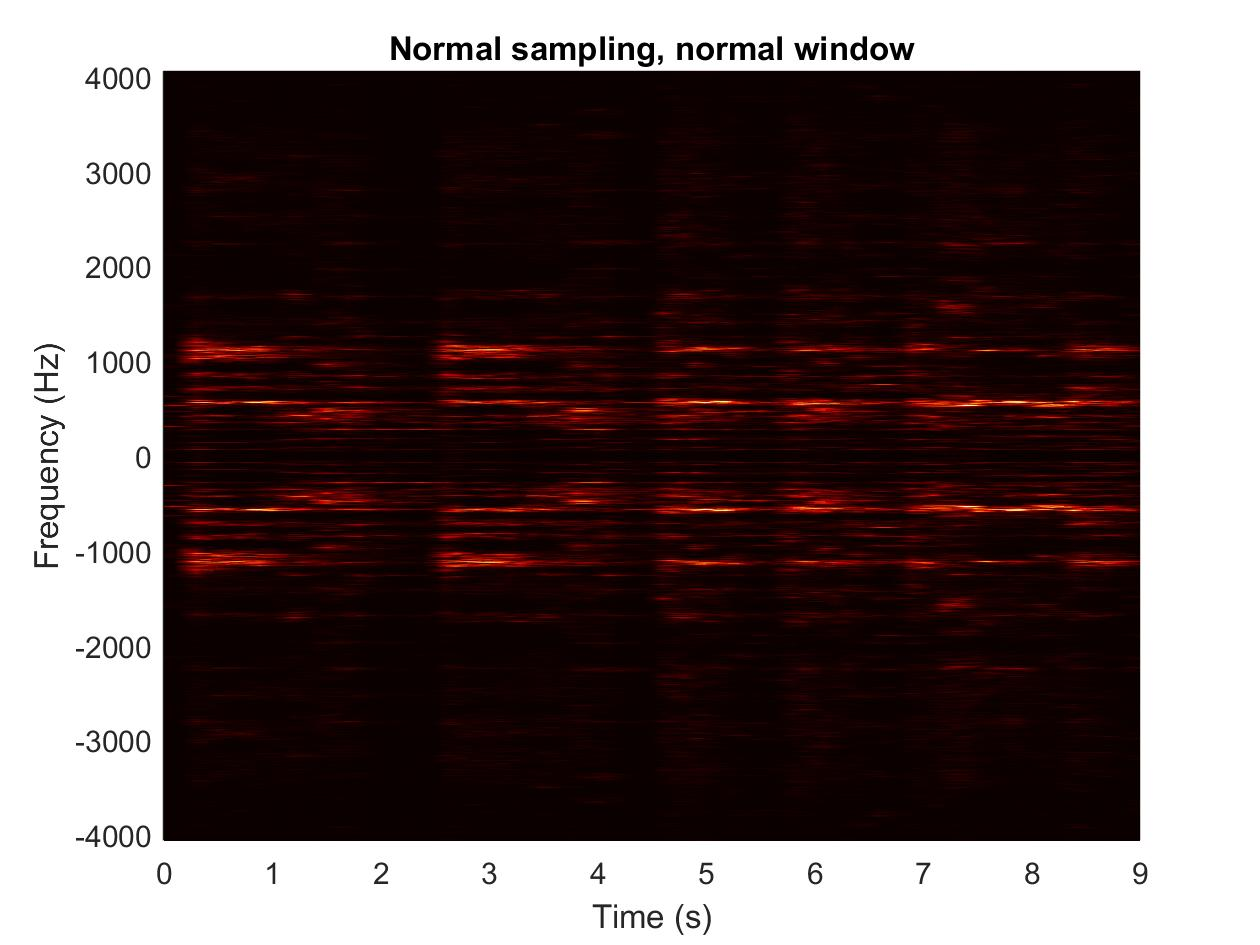
\includegraphics[width = 10cm]{normal}
\caption{\label{fig:scaled_diss} (left) Spectogram of normally made data}
\end{center}
\end{figure}


\begin{figure}
\begin{center}
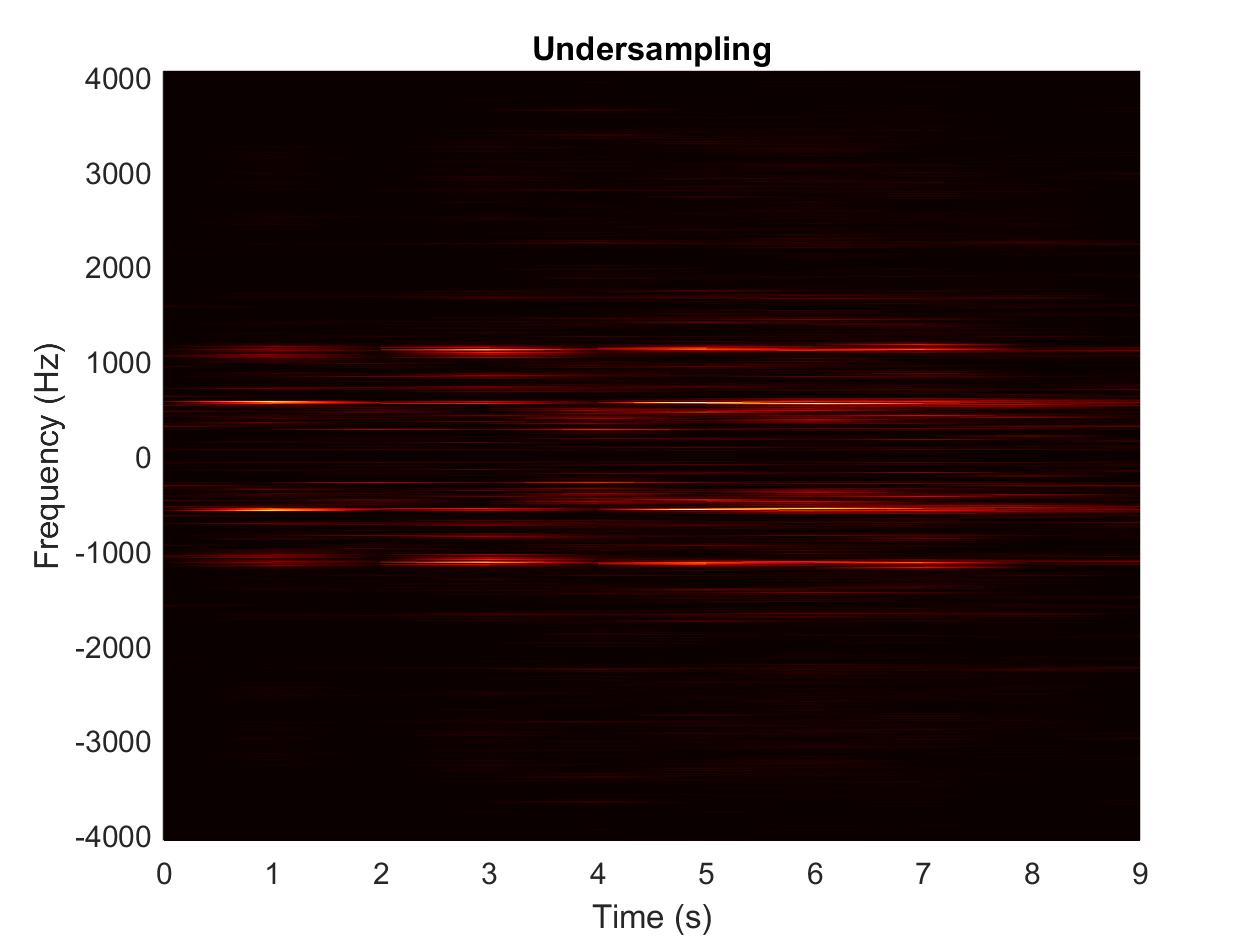
\includegraphics[width = 8cm]{undersampling}
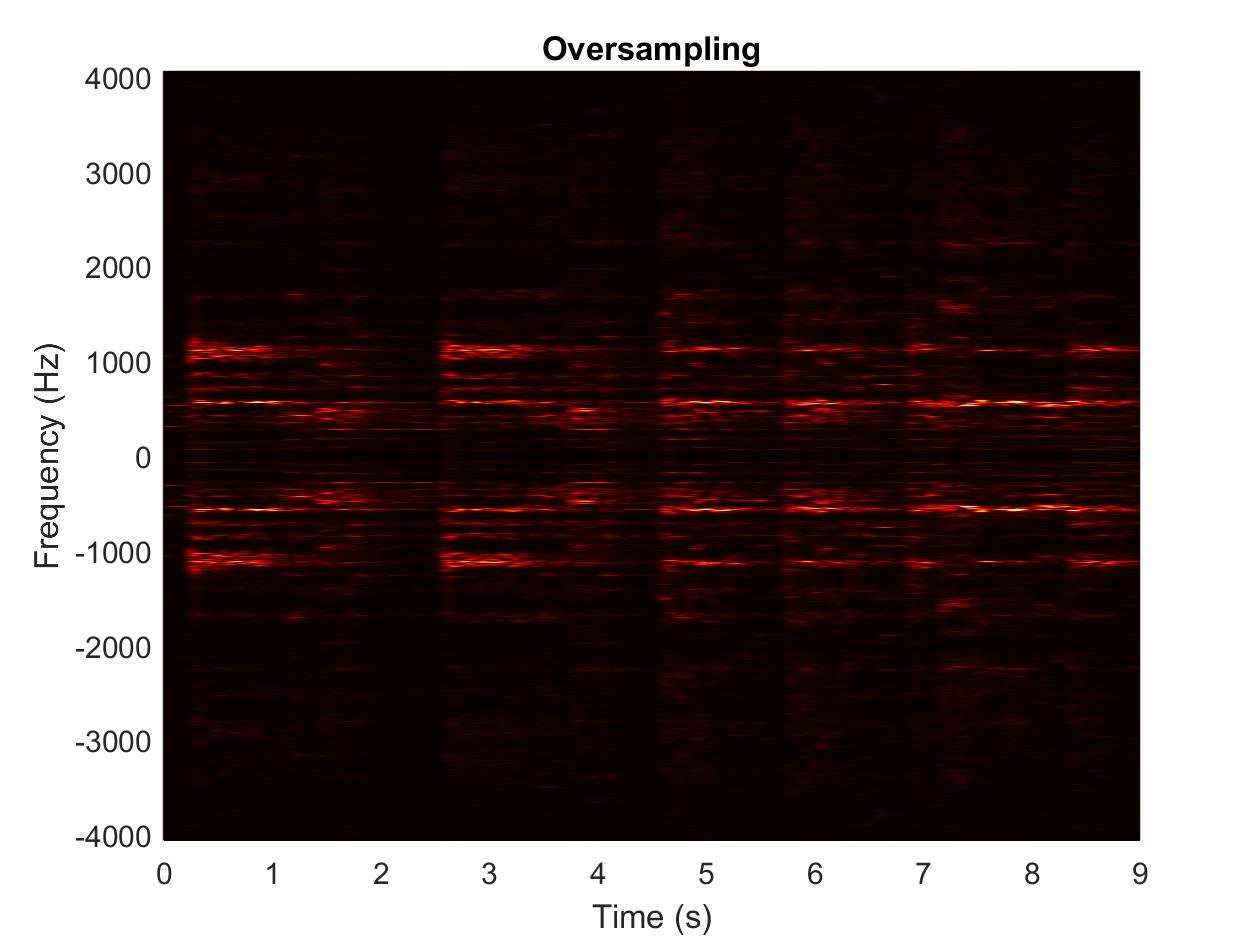
\includegraphics[width = 8cm]{oversampling}
\caption{\label{fig:scaled_diss} (left) Spectogram of Undersampled Data}
\caption{\label{fig:scaled_diss} (right) Spectogram of Oversampled Data}
\end{center}
\end{figure}

\section*{\fontsize{19}{15}\selectfont Computational Results}
	\textbf{Part One} \\
	We were able to find a balance of the correct level of accuracy in the time and frequency domain by using a value of -100 for our sigma in our Gaussian filter. We first generated a spectogram of our data using this accurate filter, as well as a reasonable sampling amount (100). We then compared it to our undersampled and oversampled data. We see that in when we undersample, the quality of the data dramatically dips, and we are left with an incoherent spectogram, both in the time and the frequency domain. Oversampling, on the other hand, produces a slightly clearer spectogram. Although this may sound good in principle, the benefits of oversampling were minimal - the spectograms of the normally sampled and oversampled data looked almost identical - the negatives were that run time severely increased because we were introducing so much more data.\\ \\
\begin{figure}[h]
\begin{center}
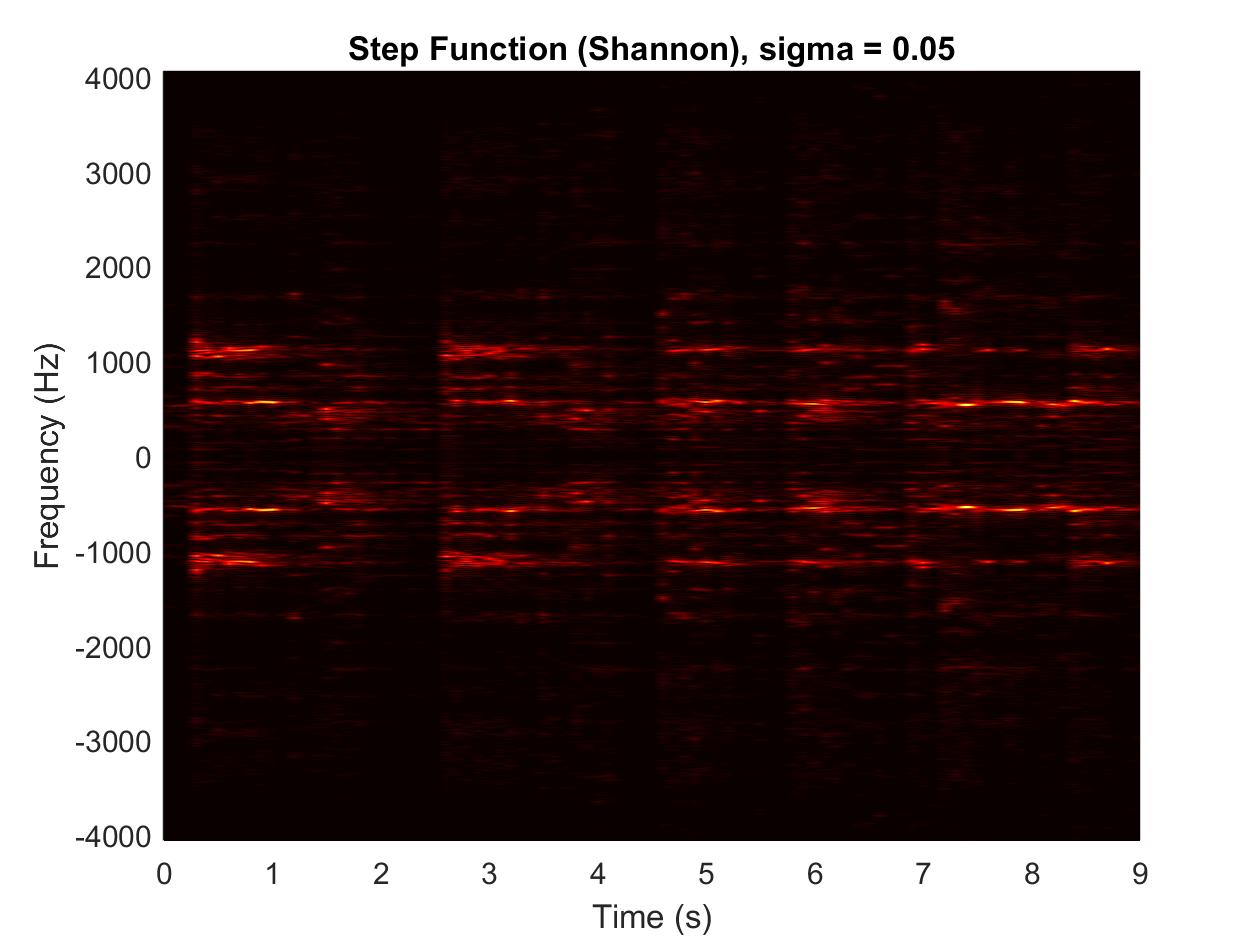
\includegraphics[width = 8cm]{shannon}
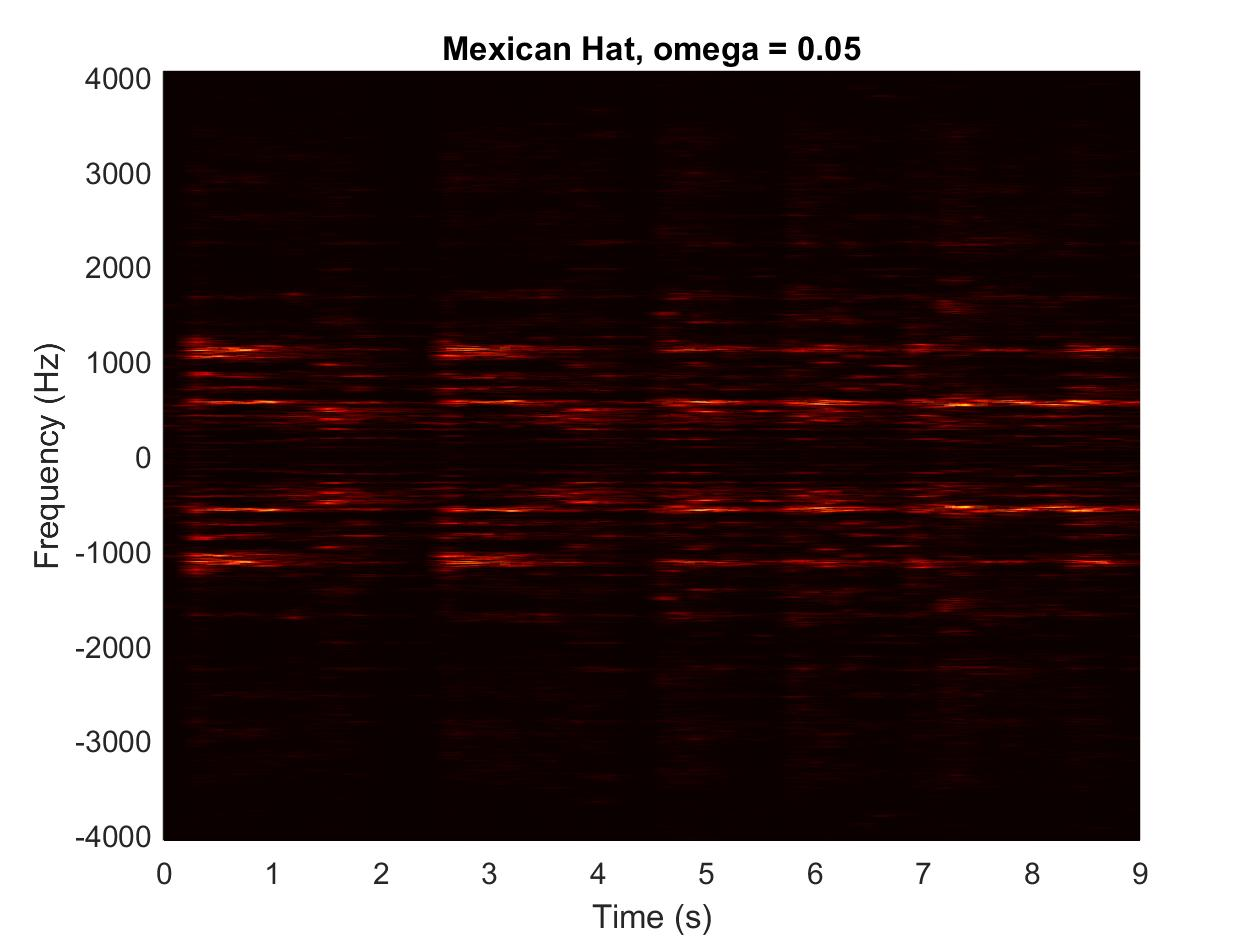
\includegraphics[width = 8cm]{mxhat}
\caption{\label{fig:scaled_diss} (left) Spectogram of Shannon Filtered Data}
\caption{\label{fig:scaled_diss} (right) Spectogram of Mexican Hat Filtered Data}
\end{center}
\end{figure}

\begin{figure}[h]
\begin{center}
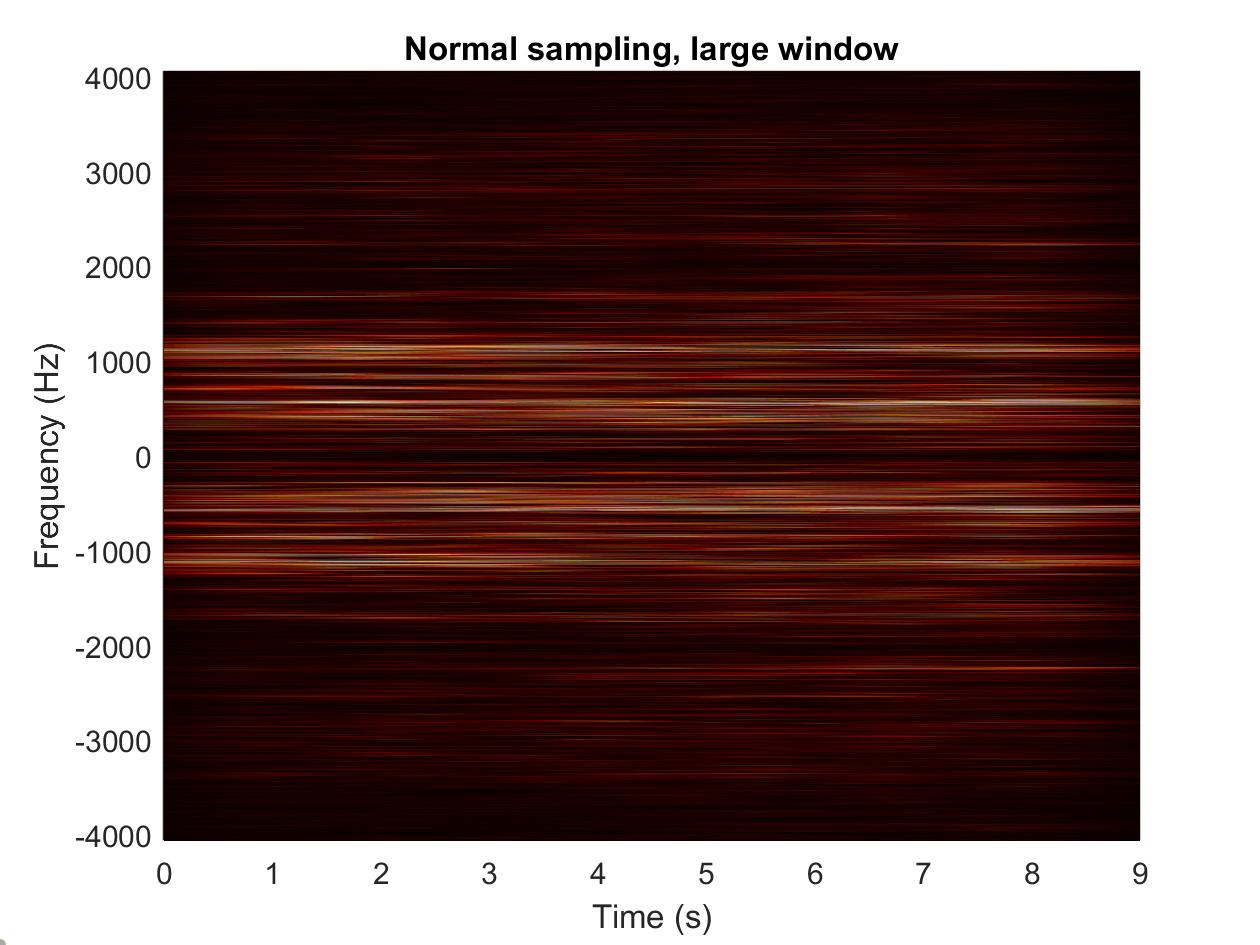
\includegraphics[width = 8cm]{largewindow}
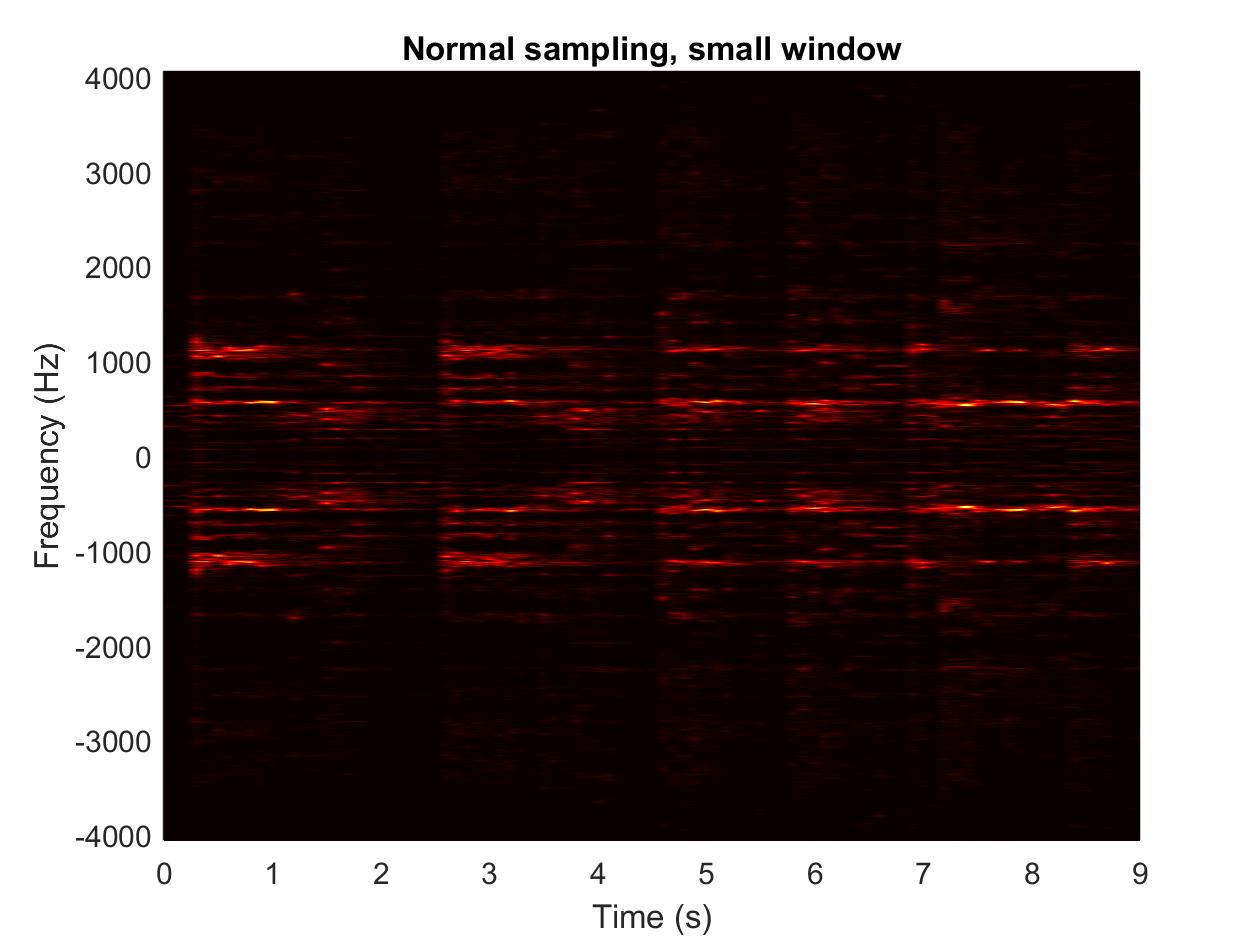
\includegraphics[width = 8cm]{smallwindow}
\caption{\label{fig:scaled_diss} (left) Spectogram of Large Window Filtered Data}
\caption{\label{fig:scaled_diss} (right) Spectogram of Small Window Filtered Data}
\end{center}
\end{figure}
We see that when we decreased the window, we got very precise measurements in the frequency domain. This is because we were essentially taking the fourier transform of a huge area, which will give us lots of information about the frequency, but not the time data. The convserse was true for a large window; We were able to see lots of information in the time domain, but because our window size was so small, we couldn't get as precise frequency measurements. \\ \\
The Mexican Hat function and Step function (Shannon) performed similarly to the Gaussian filter. We see in the spectograms that although they are similar to eachother, while the Shannon filtered data seems to have a bit more accuracy in the frequency domain at the sacrifice of less resolution in the time domain. The time domain is more continuous for the Mexican Hat filtered data, but there is less resolution in the frequency domain. However, these are both useful filters like the Gaussian filter. In both of these, we used a sigma value of 0.05, which changed the width of the filter. We also observed the same window size and undersampling/oversampling effects with these filters.

\begin{figure}[h]
\begin{center}
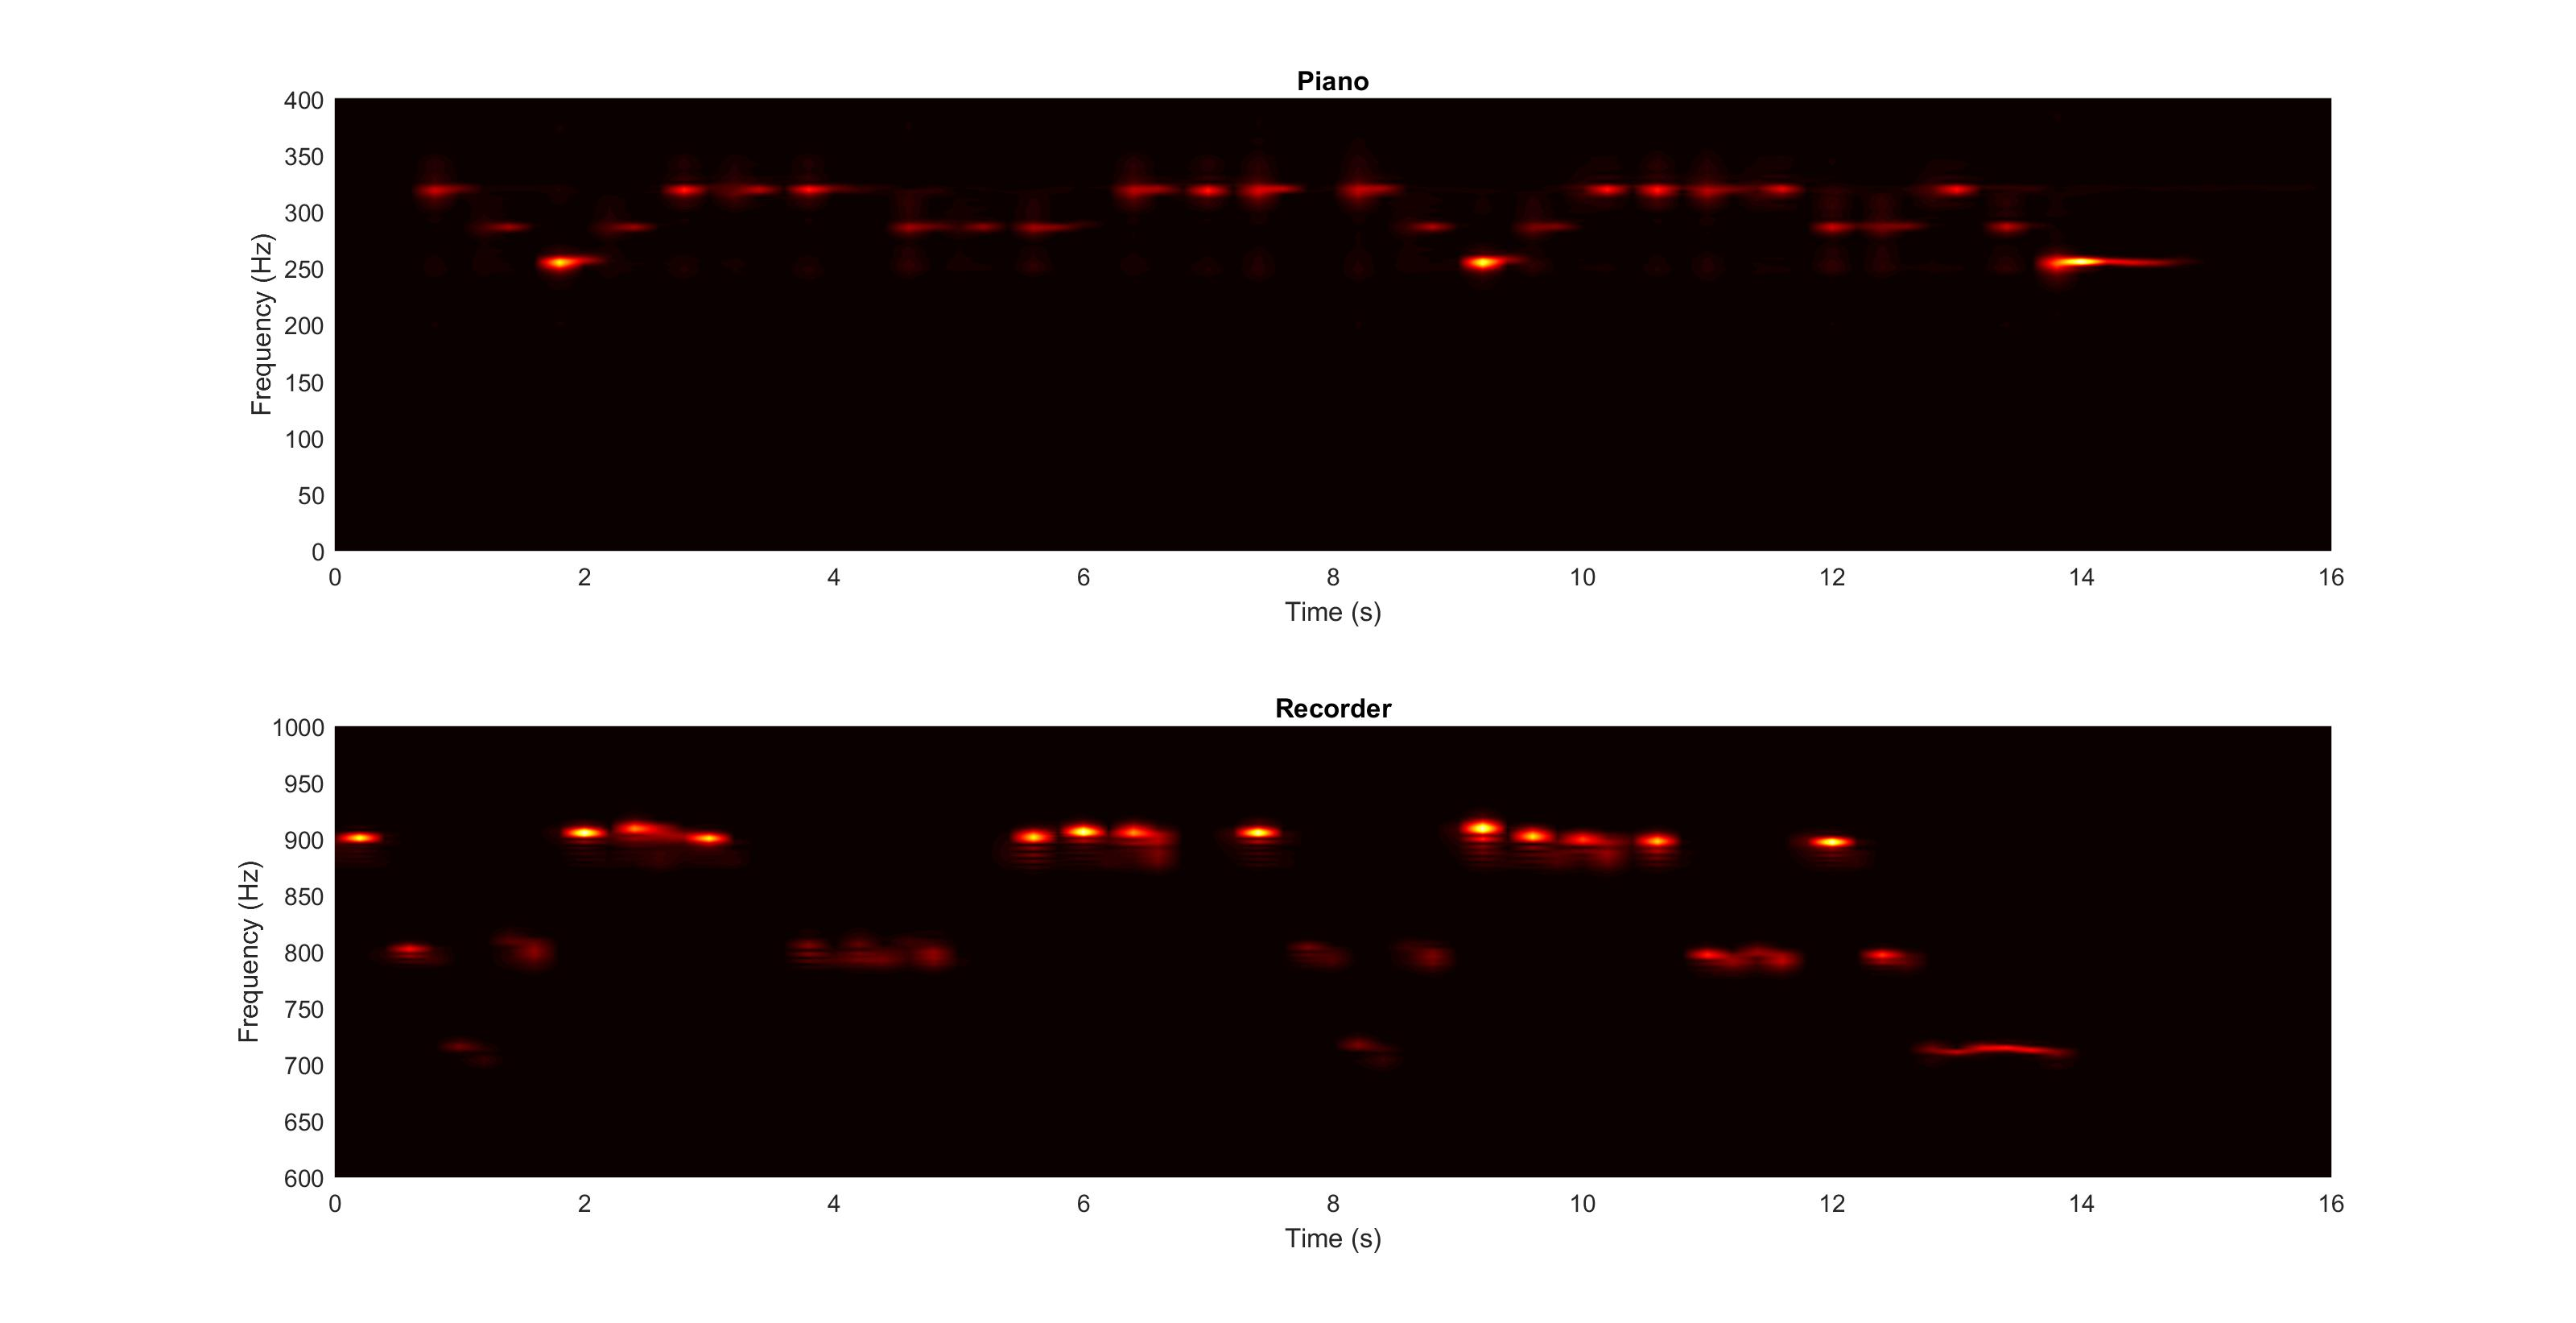
\includegraphics[width = 16cm]{pianorecorder}
\caption{\label{fig:scaled_diss} (right) Piano and Recorder Spectogram}
\end{center}
\end{figure}

\begin{figure}[h]
\begin{center}
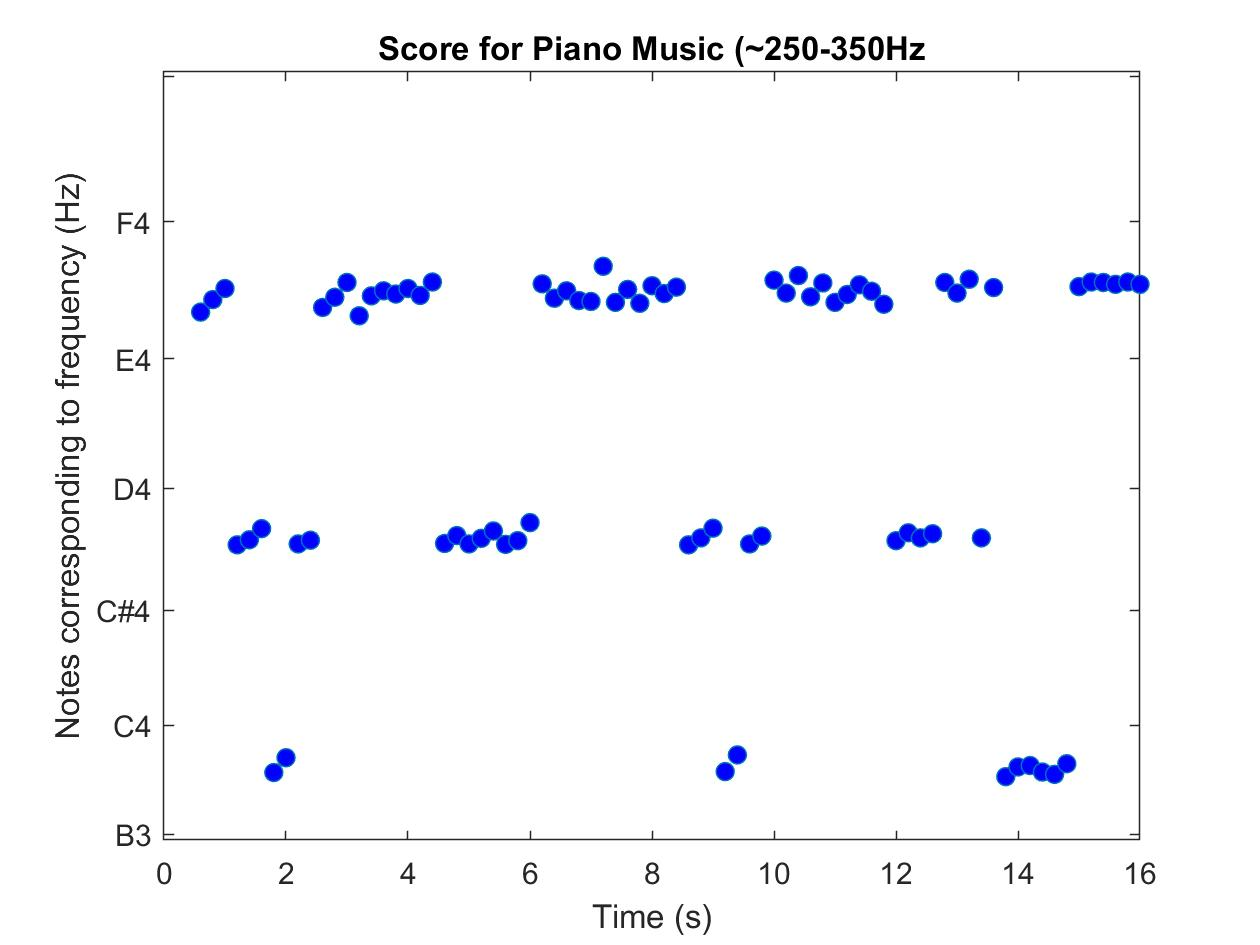
\includegraphics[width = 8cm]{piano}
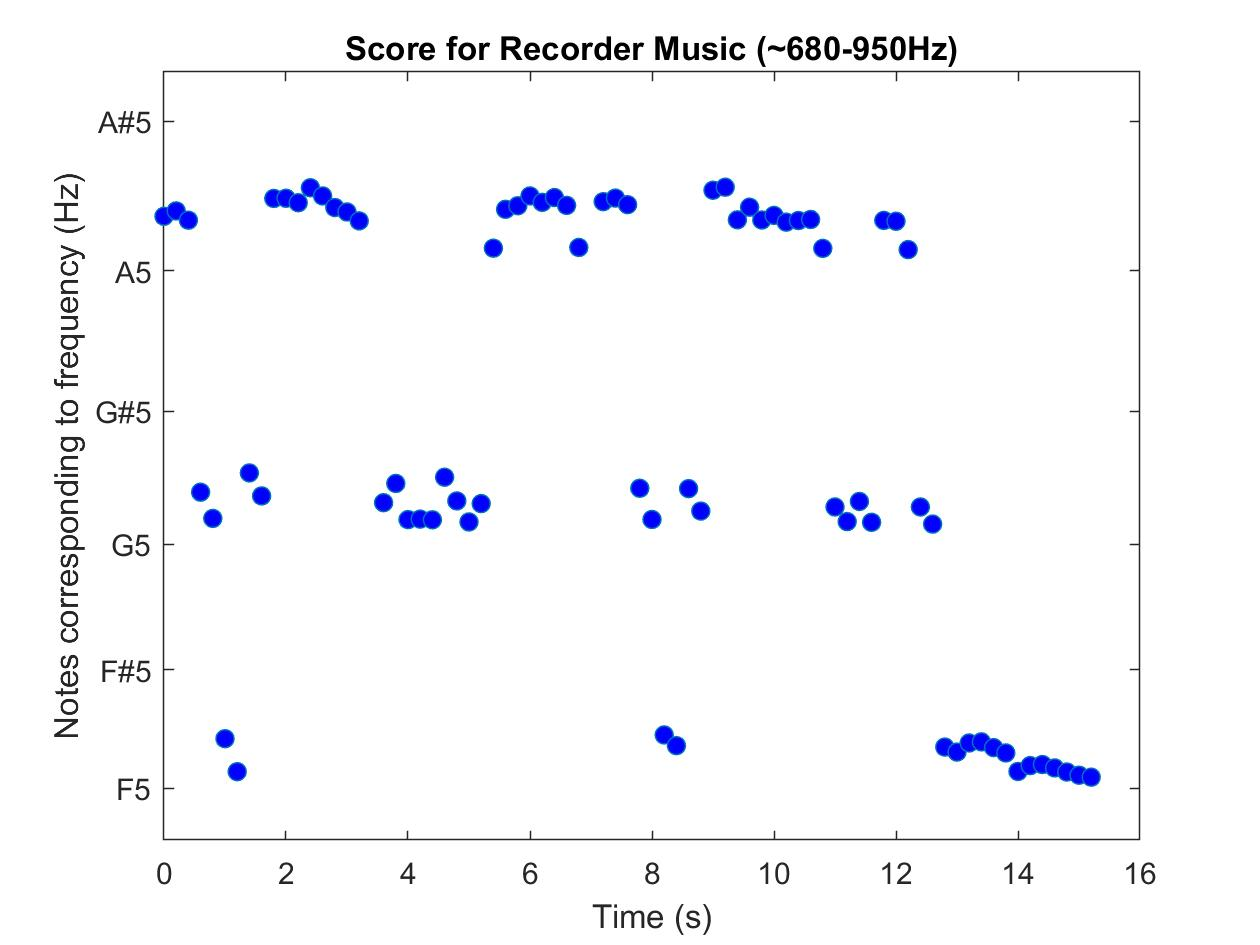
\includegraphics[width = 8cm]{recorder}
\caption{\label{fig:scaled_diss} (left) Piano Score}
\caption{\label{fig:scaled_diss} (right) Recorder Score}
\end{center}
\end{figure}
\textbf{Part Two} \\
We were able to determine the score of the music from the piano data, after filtering out overtones, and see that they follow the same general pattern, but are at different frequencies. From the spectograms of the data between the recorder and the piano, we see that there seem to be more overtones and undertones on the piano than there are in a recorder. In the case of the piano, we see that outside of the brightly colored frequency areas, there are lots of residual frequencies above and below it. In recorders, we see that most of the other frequencies seem to be below the note. 

\section*{\fontsize{19}{15}\selectfont Summary and Conclusions}
We started with music data purely in the time domain. In order to visualize this data in the time and frequency domain, we employed the Ga\'bor transform, which allowed us to create spectograms to visualize the data. We were able to see how changing parameters in the filter, as well as changing the filter itself, affected the transformation. Finally, from music data from a piano and a recorder, we took the G\'abor transform and filtered out overtones in order to reproduce the score.
\section*{\fontsize{19}{15}\selectfont Appendix A}
\subsection*{MATLAB functions used and implementation}
"abs(X)" : Returns the absolute value of every element in X, or complex magnitude if the element is complex. We used this function to normalize the data before plotting our spectogram.\\ \\
"fft(X)" : Performs a fast fourier transform on "X", a 2-D array. We used this fourier transform the filter multiplied by the data at each of our time points.\\ \\
"fftshift(X)" : Rearranges the contents of "X" by placing the zero-frequency component to the center of the array. If "X" is a vector, shifts the left and right halves of "X", while if "X" is a matrix, the $I$ and $III$ quadrants are switched, as well as the $II$ and $IV$ quadrants. We used this to change our transformed data and our axes for proper visualization.  \\ \\
"linspace(x1,x2,n)" : Creates a vector of "n" evenly spaced points from "x1" to "x2". We used this to create our linearly spaced data.  \\ \\
"[M,I] = max(A)" : Returns the maximum value "M" and the index "I"  of the matrix. We used this in part 2 to filter out the overtones by determining the index of the max value of a fourier transform of a time slice.
\pagebreak
\section*{\fontsize{19}{15}\selectfont Appendix B}
\subsection*{MATLAB code}
\begin{lstlisting}[style=Matlab-editor]
%Part One
clear all; close all; clc;
clear all; close all; clc;

load handel
v = y'/2;
v(end) = [];
vt = fft(v);

%My code
L = 9; n = length(v);
t2 = linspace(0, L, n+1); t= t2(1:n);
k = (2*pi/L) * [0:n/2-1 -n/2:-1]; ks = fftshift(k);   

subplot(2,1,1)
plot(t,v);
xlabel('Time [sec]');
ylabel('Amplitude');
title('Signal of Interest, v(n)');

subplot(2,1,2)
plot(ks, abs(fftshift(vt)));


%Gaussian Window
tslide= 0:0.1:9;
spc = [];
spcsmallwindow = [];
spclargewindow = [];
spcmxhat = [];
spcshn = [];

figure(2)
for j=1:length(tslide)
    g = exp(-100*(t-tslide(j)).^2);
    gsm = exp(-1*(t-tslide(j)).^2);
    glg = exp(-1000*(t-tslide(j)).^2);
    
    omega = 0.05;
    mxhat = (2/ (sqrt(3*omega) * pi^(0.25))).* (1-((t-tslide(j))/omega).^2) .* exp(-((t-tslide(j)).^2)/(2 * omega^2));
    
    sig = 0.05;
    shn = abs(t-tslide(j)) <= sig/2;
    
    vg = g.*v;
    vgt = fft(vg);
    
    vgsm = gsm.*v;
    vgsmt =fft(vgsm);
    
    vglg = glg.*v;
    vglgt =fft(vglg);
    
    vmx = mxhat.*v;
    vmxt = fft(vmx);
    
    vshn = shn.*v;
    vshnt = fft(vshn);
    
%     subplot(2,1,1)
%     plot(t,v,'k-', t, mxhat, 'Linewidth', 2);
%     axis([0 9 -0.5 1])
%     
%     subplot(2,1,2)
%     plot(t,vg, 'Linewidth', 2);
%     axis([0 9 -0.4 0.4])
%     
    spc = [spc; abs(fftshift(vgt))];
    spcsmallwindow = [spcsmallwindow; abs(fftshift(vgsmt))];
    spclargewindow = [spclargewindow; abs(fftshift(vglgt))];
    spcmxhat = [spcmxhat; abs(fftshift(vmxt))];
    spcshn = [spcshn; abs(fftshift(vshnt))];
    pause(0.00001);
end

tslideover = 0:0.01:9;
spcover = []
for j=1:length(tslideover)
    g = exp(-200*(t-tslideover(j)).^2);
    vg = g.*v;
    vgt = fft(vg);
    
    spcover = [spcover; abs(fftshift(vgt))];
    pause(0.00001);
end

tslideunder = 0:1:9;
spcunder = []
for j=1:length(tslideunder)
    g = exp(-200*(t-tslideunder(j)).^2);
    vg = g.*v;
    vgt = fft(vg);
    
    spcunder = [spcunder; abs(fftshift(vgt))];
    pause(0.00001);
end

figure;
%frequency here?
pcolor(tslide,ks./(2*pi),spc.'), shading interp, colormap(hot)
xlabel("Time (s)");ylabel("Frequency (Hz)"); title("Normal sampling, normal window");

figure;
pcolor(tslide,ks./(2*pi),spcsmallwindow.'), shading interp, colormap(hot)
xlabel("Time (s)");ylabel("Frequency (Hz)"); title("Normal sampling, small window");

figure;
pcolor(tslide,ks./(2*pi),spclargewindow.'), shading interp, colormap(hot)
xlabel("Time (s)");ylabel("Frequency (Hz)"); title("Normal sampling, large window");

figure;
pcolor(tslide,ks./(2*pi),spcmxhat.'), shading interp, colormap(hot)
xlabel("Time (s)");ylabel("Frequency (Hz)"); title("Mexican Hat, omega = 0.05");

figure;
pcolor(tslide,ks./(2*pi),spcshn.'), shading interp, colormap(hot)
xlabel("Time (s)");ylabel("Frequency (Hz)"); title("Step Function (Shannon), sigma = 0.05");

figure;
pcolor(tslideover,ks./(2*pi),spcover.'), shading interp, colormap(hot)
xlabel("Time (s)");ylabel("Frequency (Hz)"); title("Oversampling");

figure;
pcolor(tslideunder,ks./(2*pi),spcunder.'), shading interp, colormap(hot)
xlabel("Time (s)");ylabel("Frequency (Hz)"); title("Undersampling");

%Part Two
close all; clear all; clc;

pia=(audioread('music1.wav')).'; 
% plot((1:length(pia))/Fs,pia);
% xlabel('Time [sec]'); ylabel('Amplitude');
% title('Mary had a little lamb (piano)'); drawnow

Lpia=16;  % record time in seconds%
n = length(pia);
Fspia=length(pia)/Lpia;
t2 = linspace(0, Lpia, n+1); tpia= t2(1:n);
kpia = (2*pi/Lpia) * [0:n/2-1 -n/2:-1]; kspia = fftshift(kpia); 
tslidepia = 0:0.2:16;

spcpia = [];
pianotes = [];
for j=1:length(tslidepia)
    g = exp(-100*(tpia-tslidepia(j)).^2);
    
    vgpia = g.*pia;
    vgpiat = fft(vgpia);
    [M,I] = max(vgpiat);
    
    pianotes = [pianotes; abs(kpia(I))/(2*pi)];
    spcpia = [spcpia; abs(fftshift(vgpiat))];
end

%figure(2)
rec=(audioread('music2.wav')).'; 
% plot((1:length(rec))/Fs,rec);
% xlabel('Time [sec]'); ylabel('Amplitude');
% title('Mary had a little lamb (recorder)');

Lrec=14;  % record time in seconds
Fsrec=length(rec)/Lrec;
n = length(rec);
t2 = linspace(0, Lrec, n+1); trec= t2(1:n);
krec = (2*pi/Lpia) * [0:n/2-1 -n/2:-1]; ksrec = fftshift(krec); 
tsliderec = 0:0.2:16;

spcrec = [];
recnotes = [];
for j=1:length(tsliderec)
    g = exp(-100*(trec-tsliderec(j)).^2);
    
    vgrec = g.*rec;
    vgrect = fft(vgrec);
    
    [M,I] = max(vgrect);
    recnotes = [recnotes; abs(krec(I))/(2*pi)];
    
    spcrec = [spcrec; abs(fftshift(vgrect))];
end

% figure;
% 
subplot(2,1,1)
pcolor(tslidepia,(kspia/(2*pi)),spcpia.'), shading interp
xlabel("Time (s)");ylabel("Frequency (Hz)"); title("Piano");
ylim([0 400])
subplot(2,1,2)
pcolor(tsliderec,ksrec/(2*pi),spcrec.'), shading interp, colormap(hot)
xlabel("Time (s)");ylabel("Frequency (Hz)"); title("Recorder");
ylim([600 1000])

plot(tslidepia,pianotes,'o','MarkerFaceColor', 'b');
yticks([246.9417,261.6256,277.1826,293.6648,311.127,329.6276,349.2282]);
yticklabels({'B3','C4','C#4','D4','E4','F4'});
ylim([246 350])
title("Score for Piano Music (~250-350Hz");
xlabel("Time (s)"); ylabel("Notes corresponding to frequency (Hz)");

plot(tsliderec,recnotes,'o', 'MarkerFaceColor', 'b')
yticks([698.4565,739.9888,783.9909,830.6094,880,932.3275]);
yticklabels({'F5','F#5','G5','G#5','A5','A#5'});
ylim([680 950])
title("Score for Recorder Music (~680-950Hz)");
xlabel("Time (s)"); ylabel("Notes corresponding to frequency (Hz)");
\end{lstlisting}

\end{document}
